\chapter{Funcionamento dos Discos Rígidos}

\section{Componentes de Funcionamento}

Os discos são guardados em uma espécie de caixa, selada, que evita a entrada de material externo, tendo em vista que uma partícula de poeira pode danificar os discos altamente sensíveis.

\subsection{Discos}

O mercado apresenta tamanhos padrões de HDs, atualmente de 3.5'' para workstations e de 2.5'' para laptops. Há ainda os de 1.8'' e 1'' que são utilizados em dispositivos portáteis como players de áudio. Essas medidas se referem ao diâmetro dos discos.

\subsection{Circuito Lógico}

\subsubsection{Chip Controlador}

O circuito lógico de um HD reúne componentes responsáveis por gerenciar as ações de movimentação dos discos e das cabeças de leitura/gravação, envio e recebimento de dados entre os discos e o computador e rotinas de segurança.

\subsubsection{Chip de Buffer}

Possui a tarefa de armazenar pequenas quantidades de dados durante a comunicação com o computador, utilizado por conseguir trabalhar com os dados em uma velocidade maior que os discos rígidos ele agiliza o processo de transferência de informações.

Atualmente no mercado temos discos com capacidade de buffer entre 2 MB e 64 MB.

\subsection{Pratos e Eixo}

Os pratos são os discos onde os dados são armazenados. Geralmente feitos de alumínio ou um tipo de cristal, recoberto por material magnético e outra camada de material para proteção.

Os HDs de grande quantidade contam com a presença de vários pratos, uns sobre os outros, posicionados sob um eixo que os permite girar. Atualmente eles podem girar a velocidade de 7.200 RPM (rotações por minuto), mas já existem modelos que o fazem a 10.000 RPM. Há pouco tempo atrás o padrão era 5.400 RPM.

\subsection{Cabeça e Braço}

De tamanho bastante reduzido, contém uma bobina que utiliza impulsos magnéticos para manipular as moléculas da superfície dos pratos (discos) e assim realizar a gravação das informações nos mesmos. Há uma cabeça para cada lado do disco. Essa cabeça está posicionada na ponta de um dispositivo chamado \textbf{braço}. Sua função é posicionar as cabeças de leitura/escrita sobre a superfície dos discos.

As cabeças de leitura \textbf{não} tocam os discos fisicamente. A distância é extremamente pequena e a comunicação entre eles é feita pelos impulsos magnéticos já citados.

Em HDs atuais, o cabeçote (que contém as cabeças de gravação/leitura) contém uma cabeça para gravação e outra para leitura separadamente. Em dispositivos mais antigos isso era feito por um único componente.

\subsection{Atuador}

É o componente responsável por mover o braço acima da superfície dos discos, alcançando assim as áreas do disco para realizar as operações de leitura e gravação. O atuador possui uma bobina induzida por imãs que possibilita sua movimentação.

\section{Gravação e Leitura dos Dados}

A superfície dos pratos é composta por materiais sensíveis ao magnetismo (normalmente é utilizado óxido de ferro). O cabeçote manipula as moléculas deste material por meio de seus polos. Para isso, a polaridade das cabeças muda em uma frequência muito alta - quando está positiva, atrai o polo negativo das moléculas e vice-versa. De acordo com esta polaridade é que os bits (0 e 1) são gravados.

No processo de leitura dos dados o cabeçote efetua a leitura do campo magnético gerado pelas moléculas e gera uma corrente elétrica correspondente, cuja variação é analisada pelo controlador do HD para determinar os que foi lido.

\subsection{Organização dos Dados}

Para ordenar os dados é utilizado um esquema conhecido como ``\emph{geometria dos discos}''. Assim, o disco é divido em \textbf{cilindros}, \textbf{trilhas} e \textbf{setores}, como mostra a imagem \ref{fig:disco_divisao}.

\begin{figure}[htb]
\centering
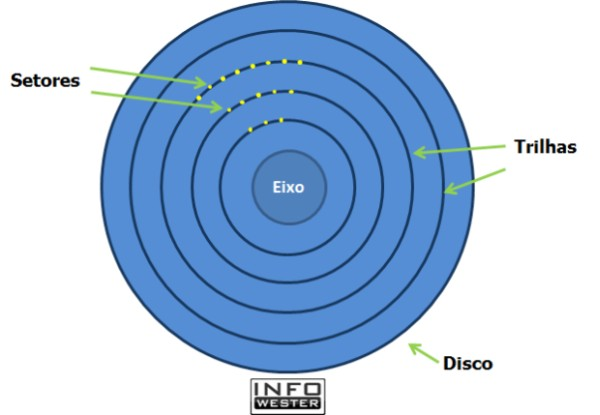
\includegraphics[width=0.8\textwidth]{hd/fig/disco_divisao.png}
\caption{Geometria dos discos}
\label{fig:disco_divisao}
\end{figure}

\subsubsection{Trilhas e Setores}

As trilhas são raios ao redor do eixo do disco que começam em sua borda e vão até o centro. Essas trilhas são numeradas a partir da borda do disco começando pela trilha 0. Cada trilha é dividida em trechos regulares chamados de setores. Cada setor possui uma capacidade determinada de armazenamento (geralmente, 512 bytes).

\subsubsection{Cilindros}

Sabe-se que o HD possui vários pratos e que há uma cabeça de leitura de gravação de cada lado do disco, e que há somente um braço de leitura para todos os discos e que se movimenta igualmente para todos os discos, quando se quer ler uma determinada trilha de um dos discos, automaticamente o cabeçote se posiciona nessa mesma trilha em todos os discos. Quando isso ocorre dá-se o nome de cilindro\footnote{Cilindro é a posição das cabeças de leitura/gravação sobre as mesmas trilhas de seus respectivos discos.}.

\subsubsection{Formatação}

Para receber os dados o disco precisa estar ``preparado''. Essa preparação é feita através da formatação. Há 2 tipos de formatação:

\begin{itemize}
	\item Física; e
	\item Lógica.
\end{itemize}

\textbf{Física}

A formatação física é a divisão do disco nas estruturas de tricas e setores. Esse procedimento é feito pelo fabricante do HD obedecendo os padrões estabelecidos.

\textbf{Lógica}

Por sua vez, esta formatação consiste na aplicação de um sistema de arquivos apropriado para cada sistema operacional. O Windows, por exemplo, é capas de trabalhar com sistemas FAT e NTFS, já o linux é capaz de trabalhar com vários sistemas de arquivos, dentre eles o ext3 e o ReiserFS.

\section{Interfaces de Comunicação}

Para se comunicar com o computador, o HD utiliza uma interface capaz de transmitir os dados entre ele e o computador de maneira segura e eficiente.

Os padrões de interface mais comuns são:

\begin{itemize}
	\item IDE;
	\item SCSI; e
	\item SATA.
\end{itemize}

\subsection{IDE(PATA)}

A interface IDE, também conhecida como \emph{\textbf{ATA}}, ligação feita através de um cabo flat (\emph{flat cable}) de 40 vias, posteriormente sendo utilizado um cabo de 80 vias cujos fios extras servem para evitar a perda de dados causadas por ruídos (interferências). A imagem \ref{fig:hd_cabo_ide} ilustra um modelo de cabo flat de 80 vias.

\begin{figure}[htb]
  \centering
  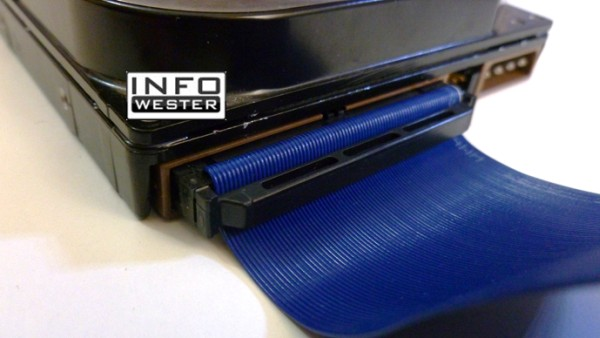
\includegraphics[width=0.8\textwidth]{hd/fig/hd_cabo_ide.jpg}
  \caption{Cabo flat de 80 vias}
  \label{fig:hd_cabo_ide}
\end{figure}

Como com o cabo flat e a conexão IDE é possível se conectar 2 HDs simultaneamente, existe um \emph{jumper} posicionado na traseira do HD que possibilita que o dispositivo (HD) possa ser identificado como sendo ``primário'' ou ``secundário''. Esse é o meio que possibilita que o computador saiba quais dados correspondem a cada dispositivo. A figura \ref{fig:hd_ide} mostra a localização do jumper no HD.

\begin{figure}[htb]
  \centering
  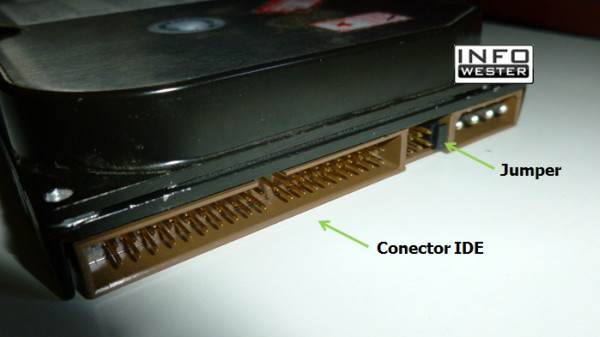
\includegraphics[width=0.8\textwidth]{hd/fig/hd_ide.jpg}
  \caption{Localização do jumper no HD}
  \label{fig:hd_ide}
\end{figure}

\newpage

A interface IDE ainda possibilita a conexão de outros dispositivos como unidades de CD/DVD. Para tal, a IDE utiliza um padrão conhecido como ATAPI que funciona como uma extensão para tornar a IDE compatível com tais dispositivos. A própria BIOS é capaz de reconhecer que tipo de aparelho está conectado em suas entradas IDE e utiliza a tecnologia correspondente (em geral, ATAPI para unidades de CD/DVD e ATA para discos rígidos).

\subsubsection{EIDE}

Uma extensão da interface IDE, possibilita a conexão simultânea de até 2 dispositivos por IDE além de aumentar a velocidade de transmissão de dados dos discos dispositivos.

\subsection{DMA e UDMA}

Antigamente, somente o processador tinha acesso direto aos dados da memória RAM. Com isso se qualquer outro componente do computador precisasse de algum dado da memória, teria que fazer acesso por intermédio do processador.

DMA (Direct Memory Access), como o próprio nome diz, tornou possível o acesso direto à memória pelo HD e outros dispositivos, sem o ``auxílio'' direto do processador.

Quando o DMA não está em uso, normalmente é utilizado um esquema de transferência de dados conhecido como PIO (Programmed I/O), onde o processador executa transferência de dados entre o HD e a memória RAM.

O UDMA permite transferência de dados a uma taxa maior que o DMA, de pelo menos 133 MB/s no caso do UDMA133, e é necessário que o chipset da placa mãe também o suporte, caso contrário, a transferência de dados será reduzida ao suportado pelo chipset da placa mãe.

\subsection{SATA}

Alcance de maiores velocidades na transferência de dados e facilidade de conexão e economia de espaço.

\begin{itemize}
  \item \textbf{SATA I}: até 150 MB/s;
  \item \textbf{SATA II}: até 300 MB/s; e
  \item \textbf{SATA III}: até 600 MB/s.
\end{itemize}

\subsection{SCSI - Small Computer System Interface}

Espercificação antiga, criada para permitir transferências de dados mais rápidas, de até 320 MB/s.

\subsection{NCQ - Native Command Queuing}

Comum nos discos rígidos atuais, o NCQ pode otimizar o desempenho do dispositivo a partir de um esquema de reorganização capaz de diminuir a carga de trabalho da unidade.

Em vez de a cabeça de leitura/gravação seguir pontos em sequência de dados ela segue a leitura conforme a proximidade dos dados, ou seja, se o ponto 3 estiver mais próximo do 1 do que o 2, a sequência de acesso será 1, 3 e 2. A figura \ref{fig:ncq} mostra a comparação de uma leitura de dados em um HD sem NCQ com um outro HD com o uso do NCQ.

\begin{figure}[htb]
  \centering
  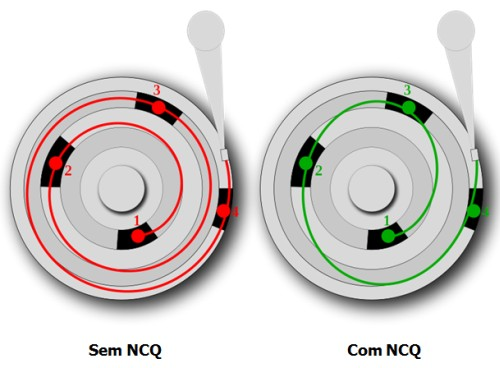
\includegraphics[width=0.8\textwidth]{hd/fig/ncq.jpg}
  \caption[Comparativo]{À esquerda um HD sem NCQ; À direita um HD com NCQ}
  \label{fig:ncq}
\end{figure}
